\begin{name}
	{\tenchude}
	{\tendethi}
	{\tentruong}
	{\thoigian}
\end{name}
\setcounter{ex}{0}\setcounter{bt}{0}
\begin{ex}%[1H4N3-1]
	Cho đường thẳng $a \subset \left(\alpha \right)$ và đường thẳng $b \subset \left(\beta \right)$. Mệnh đề nào sau đây đúng?
	\choice
	{$\left(\alpha \right) \parallel \left(\beta \right) \Rightarrow a \parallel b$}
	{\True $\left(\alpha \right) \parallel \left(\beta \right) \Rightarrow a \parallel \left(\beta \right)$ và $b \parallel \left(\alpha \right)$}
	{$a \parallel b \Rightarrow \left(\alpha \right) \parallel \left(\beta \right)$}
	{$a$ và $b$ chéo nhau}
	\loigiai{
		Do $\left(\alpha \right) \parallel \left(\beta \right)$ và $a \subset \left(\alpha\right)$ nên $a \parallel \left(\beta \right)$. Tương tự, do $\left( \alpha \right) \parallel \left(\beta \right)$ và $b \subset \left(\beta \right)$ nên $b \parallel \left(\alpha \right)$.
	}
\end{ex}

\begin{ex}%[CTST - Lớp 11 - Ôn tập cuối học kì 1 - Đề 5]%[Dương Đức]%[1D2H1-4]
	Trong các dãy số sau, dãy số nào là dãy số giảm?
	\choice
	{\True $u_n=\dfrac{2}{n^2}$}
	{$u_n=\dfrac{2n-3}{n+1}$}
	{$u_n=\dfrac{n}{3}$}
	{$u_n=\dfrac{(-1)^n}{3^n}$}
	\loigiai{
		\begin{itemize}
			\item Ta có $u_n=\dfrac{2}{n^2}\Rightarrow u_{n+1}=\dfrac{2}{(n+1)^2}$. Xét tỉ số
			      $\dfrac{u_{n+1}}{u_n}=\dfrac{n^2}{(n+1)^2}<\dfrac{n^2}{n^2}=1$.\\
			      Mà $u_n>0\Rightarrow u_n<u_{n+1},\forall n\in \mathbb{N}^{*}$. Vậy $\left(u_n\right)$ là dãy số giảm.
			\item Ta có $u_n=\dfrac{2n-3}{n+1}$; $ u_{n+1}=\dfrac{2n-1}{n+2}$.\\
			      Xét hiệu $ u_{n+1}-u_n=\dfrac{2n-1}{n+2}-\dfrac{2n-3}{n+1}=\dfrac{5}{(n+1)(n+2)}>0$ $\forall n\in \mathbb{N}^{*}$.\\
			      Vậy $\left(u_n\right)$ là dãy số tăng.
			\item Ta có $u_n=\dfrac{n}{3}$; $u_{n+1}=\dfrac{n+1}{3}$.\\
			      Xét hiệu $u_{n+1}-u_n=\dfrac{n+1}{3}-\dfrac{n}{3}=\dfrac{1}{3}>0, \forall n\in \mathbb{N}^{*}$.\\
			      Vậy $\left(u_n\right)$ là dãy số tăng.
			\item 	Ta có $u_1=\dfrac{-1}{3}$; $u_2=\dfrac{1}{9}$; $u_3=\dfrac{-1}{27}$.\\
			      Vậy $(u_n)$ là dãy số không tăng không giảm.
		\end{itemize}
	}
\end{ex}

\begin{ex}%[Pj08-0-GK1-NH23-24--TeamTeXHoa--LeQuan]%[1D3N2-1]
	Cho $\lim\limits_{x\to{x_0}}f(x)=L\,\left(L > 0\right)$ , $\lim\limits_{x\to{x_0}}g(x)=0\,\left(g(x) < 0,\,\forall x\ne{x_0}\right)$. Mệnh đề nào sau đây đúng?
	\choice
	{$\lim\limits_{x\to{x_0}}\dfrac{f(x)}{g(x)}=+\infty $}
	{\True $\lim\limits_{x\to{x_0}}\dfrac{f(x)}{g(x)}=-\infty $}
	{$\lim\limits_{x\to{x_0}}\dfrac{f(x)}{g(x)}=0$}
	{$\lim\limits_{x\to{x_0}}\dfrac{f(x)}{g(x)}=L$}
	\loigiai{
		Ta có   $\lim\limits_{x\to{x_0}}f(x)=L\,\left(L > 0\right)$, $\lim\limits_{x\to{x_0}}g(x)=0\,\left(g(x) < 0,\,\forall x\ne{x_0}\right)$ thì $\lim\limits_{x\to{x_0}}\dfrac{f(x)}{g(x)}=-\infty $.}
\end{ex}

\begin{ex}%[1D3N3-1]
	Cho hàm số $y=f(x)$ liên tục trên $(a;b)$. Điều kiện cần và đủ để hàm số liên tục trên $[a;b]$ là
	\choice
	{$\lim\limits_{x\to a^+}f(x)=f(a)$ và $\lim\limits_{x\to b^+}f(x)=f(b)$}
	{\True $\lim\limits_{x\to a^+}f(x)=f(a)$ và $\lim\limits_{x\to b^-}f(x)=f(b)$}
	{$\lim\limits_{x\to a^-}f(x)=f(a)$ và $\lim\limits_{x\to b^+}f(x)=f(b)$}
	{$\lim\limits_{x\to a^-}f(x)=f(a)$ và $\lim\limits_{x\to b^-}f(x)=f(b)$}
	\loigiai{
		Cho hàm số $y=f(x)$ liên tục trên $(a;b)$. Điều kiện cần và đủ để hàm số liên tục trên $[a;b]$ là $\lim\limits_{x\to a^+}f(x)=f(a)$ và $\lim\limits_{x\to b^-}f(x)=f(b)$.
	}
\end{ex}

\begin{ex}%[1D5N1-2]%[Dự án đề kiểm tra Toán 11 GHKI NH23-24- Nguyễn Văn Sang]%[ĐỀ KNTT SỐ 5]
	Mẫu số liệu sau cho biết cân nặng của học sinh lớp $12$ trong một lớp
	\begin{center}
		\begin{tabular}{|c|c|c|c|}
			\hline Cân nặng $(\mathrm{kg})$ & Dưới $55$ & Từ $55$ đến $65$ & Trên $65$ \\
			\hline Số học sinh              & $23$      & $15$             & $2$       \\
			\hline
		\end{tabular}
	\end{center}
	Số học sinh của lớp đó là bao nhiêu?
	\choice
	{\True $40$}
	{$35$}
	{$23$}
	{$38$}
	\loigiai{
		Số học sinh của lớp là $n=23+15+2=40$ học sinh.
	}
\end{ex}

\begin{ex}%[1H4N1-3]%[Dự án đề ôn tập khối 11 HKI NH2023-2024-Đơt 1-TheHung Nguyen]%[CD-Đề số 1]
	\immini{Cho hình chóp $S.ABCD$, đáy $A B C D$ là hình bình hành tâm $O$. Giao tuyến của hai mặt phẳng $(S A C)$ và $(S A D)$ là
		\choice
		{$S O$}
		{$S D$}
		{\True $SA$}
		{$S B$}}{\begin{tikzpicture}[scale=.5, font=\footnotesize, line join=round, line cap=round, >=stealth]
			\def\a{3}
			\def\b{2.5}
			\def\h{3.5}
			\def\g{35}
			\path
			(0,0) coordinate (A)
			(0:\a) coordinate (B)
			--++(\g:\b) coordinate (C)
			--++(180:\a)coordinate (D)
			;
			\coordinate (O) at ($(A)!1/2!(C)$);
			\coordinate (S) at ($(O)+(0,\h)$);
			\draw (S)--(A)--(B)--(C) (B)--(S)--(C);
			\draw[dashed] (B)--(D)--(S)--(O)  (A)--(D)--(C)--(A);
			\foreach \x/\g in {A/-90,B/-90,C/0,D/180,S/90,O/-90}  \fill (\x) circle (1pt)+(\g:.25)node {$\x$};
		\end{tikzpicture}}

	\loigiai{Ta có $(SAC)\cap(SAD)=SA$.
	}
\end{ex}

\begin{ex}%[1D1N4-2]
	Tập xác định của hàm số $y=\cot x$ là
	\choice
	{$D=\mathbb{R}$}
	{$D=\mathbb{R}\setminus\left\{\dfrac{\pi}{2}+k \pi \mid k \in \mathbb{Z}\right\}$}
	{\True $D=\mathbb{R}\setminus\{k \pi \mid k \in \mathbb{Z}\}$}
	{$D=\mathbb{R}\setminus\{0\}$}
	\loigiai{
		Ta có $y=\dfrac{\cos x}{\sin x}$, nên hàm số xác định khi $\sin x \neq 0 \Leftrightarrow x \neq k \pi$, $k \in \mathbb{Z}$.
	}
\end{ex}

\begin{ex}%[1H4N6-1]%[Pj10-1-HK1-NH23-24-TeamTeXHoa-VUNgocHao]
	Khẳng định nào sau đây {\bf sai}?
	\choice
	{Phép chiếu song song biến ba điểm thẳng hàng thành ba điểm thẳng hàng và không làm thay đổi thứ tự ba điểm đó.}
	{\True Phép chiếu song song luôn biến hai đường thẳng song song thành hai đường thẳng song song}
	{Hình biểu diễn của một hình tròn qua phép chiếu song song có thể là một hình elip}
	{ Hình chiếu song song của một đường thẳng là một đường thẳng}
	\loigiai{
		Phép chiếu song song biến hai đường thẳng song song thành hai đường thẳng song song hoặc trùng nhau.	}
\end{ex}

\begin{ex}%[Pj10-1-GK1-NH23-24--TeamTeXHoa--Lâm Chính]%[1H4N2-2]
	\immini{
		Cho hình chóp $S.ABCD$ có đáy $ABCD$ là hình bình hành. Gọi $I$, $J$, $E$, $F$ lần lượt là trung điểm $SA$, $SB$, $SC$, $SD$. Trong các đường thẳng sau, đường thẳng nào \textbf{không} song song với $IJ$?
		\choice
		{\True $AD$}
		{$AB$}
		{$EF$}
		{$DC$}
	}{
		\begin{tikzpicture}[scale=0.6, font=\footnotesize,line join=round, line cap=round, >=stealth]
			\coordinate (A) at (0,0);
			\coordinate (B) at (-2,-2);
			\coordinate (D) at (4,0);
			\coordinate (C) at ($(B)+(D)-(A)$);
			\coordinate (H) at ($(A)!0.4!(B)$);
			\coordinate (S) at ($(H)+(0,4)$);
			\coordinate (I) at ($(S)!0.5!(A)$);
			\coordinate (J) at ($(S)!0.5!(B)$);
			\coordinate (E) at ($(S)!0.5!(C)$);
			\coordinate (F) at ($(S)!0.5!(D)$);
			\foreach \i in {B,C,D}{\draw (S)--(\i);}
			\draw (B)--(C)--(D) (J)--(E)--(F);
			\draw[dashed,thin](S)--(A) (B)--(A)--(D) (F)--(I)--(J);
			\foreach \i/\g in {S/90,A/-90,B/-90,C/-90,D/-90,I/180,J/180,E/90,F/90}{\draw[fill=black](\i) circle (1.5pt) ($(\i)+(\g:4mm)$) node[scale=1]{$\i$};}
		\end{tikzpicture}}

	\loigiai{
		Ta có $IJ \parallel AB \parallel EF$, nhưng $AB\cap AD=A$ nên $IJ$ không song song với $AD$.

	}
\end{ex}

\begin{ex}%[1D3N1-1]%[Dự án đề kiểm tra Toán 11 HHKI NH23-24- Phạm Văn Long]%[Thi thử - KNTT]
	Cho hai dãy $\left(u_n \right)$ và $\left(v_n \right)$ thỏa mãn $\lim \limits{n \to +\infty}u_n=2$ và $\lim \limits{n \to +\infty}v_n=3$. Giá trị của $\lim \limits{n \to +\infty}\left(u_n+v_n \right)$ bằng
	\choice{\True $5$}
	{$6$}
	{$-1$}
	{$1$}
	\loigiai{
		Ta có $\lim \limits{n \to +\infty}\left(u_n+v_n \right)=\lim \limits{n \to +\infty}u_n+\lim \limits{n \to +\infty}v_n=2+3=5$.
	}
\end{ex}

\begin{ex}%[Dự án TeX GKI 11, Đoàn Hùng]%[1D2N3-1]
	Cho cấp số nhân $\left(u_n\right)$ có công bội $q$. Mệnh đề nào sau đây đúng?
	\choice
	{\True $u_n=u_1 \cdot q^{n-1}(n \geq 2)$}
	{ $u_n=u_1 \cdot q^{n+1}(n \geq 2)$}
	{ $u_n=u_1 \cdot q^{n}(n \geq 2)$}
	{ $u_n=q^{n}(n \geq 2)$}
	\loigiai{
		Mệnh đề đúng là $u_n=u_1 \cdot q^{n-1}(n \geq 2)$.
	}
\end{ex}

\begin{ex}%[1D1N3-1]%[KNTT - Lớp 11 - Ôn tập cuối học kì 1 - Đề 5]%[Võ Thanh Hiệp]
	Với $x$ là góc bất kỳ và các biểu thức có nghĩa. Đẳng thức nào dưới đây đúng?

	\choice
	{$\sin 2x = 2 \sin x \cos x$}
	{\True $\sin 2x = \sin x \cos x$}
	{$\sin 2x = 2 \cos x$}
	{$\sin 2x = 2 \sin x$}
	\loigiai
	{
		Ta có	$\sin 2x = \sin x \cos x$ đúng.
	}
\end{ex}

\begin{ex}%[1D3N1-2]%[Dự án đề kiểm tra Toán 11 GHKI NH23-24- Nguyễn Văn Sang]%[ĐỀ KNTT SỐ 5]
	Giá trị của $\lim \limits{n \to +\infty}\dfrac{2}{n^2+1}$ bằng
	\choice
	{\True $0$}
	{$2$}
	{$1$}
	{$+\infty$}
	\loigiai{
		Ta có $\lim \limits{n \to +\infty}\dfrac{2}{n^2+1}=\lim \limits{n \to +\infty}\dfrac{1}{n^2}\cdot \dfrac{2}{1+\tfrac{1}{n^2}}=0\cdot 2=0$.
	}
\end{ex}

\begin{ex}%[Pj10-0-GK1-NH23-24--TeamTeXHoa--VoVanTu]%[1H4N4-1]
	Cho ba mặt phẳng phân biệt $(\alpha);\,(\beta);\,(\gamma)$ có $(\alpha)\cap(\beta)=d_1$; $(\beta)\cap(\gamma)=d_2$; $(\alpha)\cap(\gamma)=d_3$. Khi đó ba đường thẳng $d_1$, ${d_2}$, ${d_3}$
	\choice
	{đôi một cắt nhau}
	{\True đôi một song song hoặc đồng quy}
	{đôi một song song}
	{đồng quy}
	\loigiai{
		Đáp án là đôi một song song hoặc đồng quy.}
\end{ex}

\begin{ex}%[1D1N5-1]%[Dự án đề kiểm tra Toán 11 HKI NH23-24- Tư Đô Nguyên]%[Đề 11 - CTST]
	Phương trình $\sin x=\sin\alpha $ có các nghiệm là
	\choice
	{\True $x=\alpha+k 2 \pi, x=\pi-\alpha+k 2 \pi, k \in \mathbb{Z}$}
	{$x=\alpha+k 2 \pi, x=-\alpha+k 2 \pi, k \in \mathbb{Z}$}
	{$x=\alpha+k \pi, x=\pi-\alpha+k \pi, k \in \mathbb{Z}$}
	{$x=\alpha+k \pi, x=-\alpha+k \pi, k \in \mathbb{Z}$}
	\loigiai{
		Ta có $\sin x=\sin\alpha \Leftrightarrow \hoac{&x=\alpha+k 2 \pi \\ &x=\pi-\alpha+k 2 \pi,}\, k \in \mathbb{Z}.$
	}
\end{ex}


\begin{ex}%[Pj10-1-HK1-NH23-24--TeamTeXHoa--Paul Hieu Nguyen]%[1D2H2-3]
	Cho cấp số cộng $(u_n)$ biết $u_1=5$ và $u_5=13$. Tìm $u_n$.
	\choice
	{$u_n=5n-3$}
	{$u_n=3n+2$}
	{\True $u_n=2n+3$}
	{$u_n=5n$}
	\loigiai{
		Ta có $u_5=u_1+4d\Leftrightarrow 13=5+4d\Leftrightarrow d=2$.\\
		Do đó $u_n=u_1+\left(n-1\right)d=5+2\left(n-1\right)=2n+3$.}
\end{ex}

\begin{ex}%[1D5H1-4]
	Tìm hiểu thời gian hoàn thành một bài tập (đơn vị: phút) của một số học sinh thu được kết quả sau
	\begin{center}
		\begin{tabular}{|c|c|c|c|c|c|}
			\hline\begin{tabular}{l}
				      Thời gian(giờ)
			      \end{tabular} & {$[0;4)$} & {$[4;8)$} & {$[8;12)$} & {$[12;16)$} & {$[16;20)$} \\
			\hline Số học sinh       & $2$       & $4$       & $7$        & $4$         & $3$    \\
			\hline
		\end{tabular}
	\end{center}
	Mốt của mẫu số liệu ghép nhóm này là
	\choice
	{$M_o=12$}
	{$M_o=11$}
	{\True $M_o=10$}
	{$M_o=9$}
	\loigiai{Nhóm chứa Mốt của bảng số liệu này là $[8;12)$, suy ra Mốt của bảng số liệu là
	\[M_o=8+\dfrac{7-4}{(7-4)+(7-4)}\cdot(12-8)=10.\]}
\end{ex}

\begin{ex}%[1D5H1-3]%[Dự án đề kiểm tra Toán 11 GHKI NH23-24- Nguyễn Văn Sang]%[ĐỀ KNTT SỐ 5]
	Cân nặng của $28$ học sinh của một lớp $11$ được cho như sau
	\begin{center}
		\begin{tabular}{*{14}{c}}
			55{,}4 & 62{,}6 & 54{,}2 & 56{,}8 & 58{,}8 & 59{,}4 & 60{,}7 & 58     & 59{,}5 & 63{,}6 & 61{,}8 & 52{,}3 & 63{,}4 & 57{,}9 \\
			49{,}7 & 45{,}1 & 56{,}2 & 63{,}2 & 46{,}1 & 49{,}6 & 59{,}1 & 55{,}3 & 55{,}8 & 45{,}5 & 46{,}8 & 54     & 49{,}2 & 52{,}6 \\
		\end{tabular}
	\end{center}
	Số trung bình của mẫu số liệu ghép nhóm trên xấp xỉ bằng
	\choice
	{\True $55{,}6$}
	{$65{,}5$}
	{$48{,}8$}
	{$57{,}7$}
	\loigiai{
	Khoảng biến thiên của mẫu số liệu trên là $R=63{,}6-45{,}1 = 18{,}5 $.\\
	Độ dài mỗi nhóm là $L>\dfrac{R}{k}=3{,}7 $.\\
	Ta chọn $L=4{,}0$ và chia dữ liệu thành các nhóm và có bảng giá trị đại diện như sau
	\begin{center}
		\begin{tabular}{|l|c|c|c|c|c|}
			\hline
			Nhóm             & $[45 ; 49 )$ & $[49 ; 53 )$ & $[53 ; 57 )$ & $[57 ; 61 )$ & $[61 ; 65 )$ \\
			\hline
			Giá Trị Đại Diện & $47 $        & $51 $        & $55 $        & $59 $        & $63 $        \\
			\hline
			Tần Số           & $ 4$         & $5$          & $7$          & $7$          & $5$          \\
			\hline
		\end{tabular}
	\end{center}
	Giá trị trung bình của bảng số liệu là
	\[\overline{x}=\dfrac{4 \cdot 47 + 5 \cdot 51 + 7 \cdot 55 + 7 \cdot 59 + 5 \cdot 63{,}0}{28} \approx 55{,}57.\]
	}
\end{ex}

\begin{ex} %[1D3H2-2]
	$A=\underset{x\to 2}{\mathop{\lim \limits{n \to +\infty}}}\,( x^3-18x^2+2 )$ có giới hạn hữu hạn là
	\choice
	{\True $-62$}
	{ $-15$}
	{ $62$}
	{ $15$}
	\loigiai{
	$A=\underset{x\to 2}{\mathop{\lim \limits{n \to +\infty}}}\,( x^3-18x^2+2 )=\underset{x\to 2}{\mathop{\lim \limits{n \to +\infty}}}\,x^3-\underset{x\to 2}{\mathop{\lim \limits{n \to +\infty}}}\,18x^2+\underset{x\to 2}{\mathop{\lim \limits{n \to +\infty}}}\,2=2^3-{18\cdot 2^2}+2=-62$.} \end{ex}

\begin{ex}%[1H4H1-4]
	%\immini{
	Cho hình chóp $S.ABCD$ có đáy $ABCD$ là hình bình hành tâm $O$. Gọi $M$, $N$, $K$ lần lượt là trung điểm của $CD$, $CB$, $SA$. Gọi $H$ là giao điểm của $AC$ và $MN$. Giao điểm của $SO$ với $(MNK)$ là điểm $E$. Khi đó
	\choice
	{$E$ là giao của $M N$ với $SO$}
	{$E$ là giao của $K N$ với $SO$.}
	{\True $E$ là giao của $K H$ với $SO$}
	{$E$ là giao của $K M$ với $SO$}
	\loigiai{
		\immini{		Trong mặt phẳng $(SAC)$, gọi $E=KH \cap SO$.\\
			Khi đó $\heva{&E \in KH \subset (KMN)\\ &E \in SO} \Rightarrow E=SO \cap (KMN)$.}
		{		 \begin{tikzpicture}[scale=0.8, font=\footnotesize,line join=round, line cap=round, >=stealth]
				\coordinate (A) at (0,0);
				\coordinate (B) at (-2,-2);
				\coordinate (D) at (5,0);
				\coordinate (C) at ($(B)+(D)-(A)$);
				\coordinate (O) at ($(A)!0.5!(C)$);
				\coordinate (S) at ($(O)+(0,5)$);
				\coordinate (M) at ($(C)!0.5!(B)$);
				\coordinate (N) at ($(D)!0.5!(C)$);
				\coordinate (K) at ($(S)!0.5!(A)$);
				\coordinate (H) at ($(M)!0.5!(N)$);
				\coordinate (E) at (intersection of K--H and S--O);
				\\foreach \\i in {A,B,C,D}{\\draw (S)--(\\i);}
				\\draw (B)--(C)--(D);
				\\draw[dashed,thin](S)--(A)--(B)--(D)--(A)--(C);
				\draw(S)--(B) (S)--(C) (N)--(S)--(D) (B)--(C)--(D);
				\draw[dashed,thin](S)--(A)--(C)--(M) (A)--(B) (A)--(D)--(B) (S)--(O) (A)--(N)--(M)--(K)--(N) (K)--(H);
				\foreach \i/\g in {S/90,A/-90,B/-90,C/-90,D/-90,O/-90,M/-90,N/0,K/-150,H/-90,E/180}{\draw[fill=black](\i) circle (1.5pt) ($(\i)+(\g:4mm)$) node[scale=1]{$\i$};}
			\end{tikzpicture}}
	}
\end{ex}

\begin{ex}%[1D2H2-6]
	Một đồng hồ đánh giờ, khi kim giờ chỉ số $n$ (từ $1$ đến $12$) thì đồng hồ đánh đúng $n$ tiếng. Hỏi trong một ngày ($24$ giờ) đồng hồ đánh được bao nhiêu tiếng?
	\choice
	{\True $156$}
	{$152$}
	{$148$}
	{$160$}
	\loigiai{
		Số tiếng đồng hồ đánh trong một ngày là\\
		$S=2\left(1+2+\ldots+12\right)=2\cdot \dfrac{12\cdot 13}{2}=156$.}
\end{ex}

\begin{ex}%[BG 11 - Nguyen Huynh]%[1D1N4-3]
	Phát biểu nào sau đây là đúng?
	\choice{Hàm số $y=\sin x$ nghịch biến trên $\left(\pi ; 2\pi\right)$}
	{Hàm số $y=\tan x$ đồng biến trên $(0; \pi)$}
	{Hàm số $y=\cot x$ đồng biến trên $\left[0;\pi \right]$}
	{\True Hàm số $y=\tan x$ đồng biến trên mỗi khoảng $\left(0;\dfrac{\pi}{2}\right)$, $\left(\dfrac{\pi}{2};\pi\right)$}
	\loigiai{
		Hàm số $y=\tan x$ đồng biến trên mỗi khoảng $\left(0;\dfrac{\pi}{2}\right)$; $\left(\dfrac{\pi}{2};\pi\right)$.
	}
\end{ex}

\begin{ex}%[1H4H2-2]
	Cho hình chóp $S.ABCD$ có đáy là hình bình hành. Gọi $G_1$, $G_2$ lần lượt là trọng tâm của $\triangle SAB$, $\triangle SAD$. Khi đó, $G_1G_2$ song song với đường thẳng nào sau đây?
	\choice
	{$AC$}
	{$BC$}
	{$SO$}
	{\True $BD$}
	\loigiai{
		\immini{Gọi $N$ là trung điểm của $SA$.\\
			Vì $G_1$, $G_2$ lần lượt là trọng tâm của $\triangle SAB$, $\triangle SAD$ nên ta có\\ $\dfrac{NG_1}{NB}=\dfrac{NG_2}{ND}=\dfrac{1}{3}$ $\Rightarrow$ $G_1G_2\parallel BD$.}
		{
			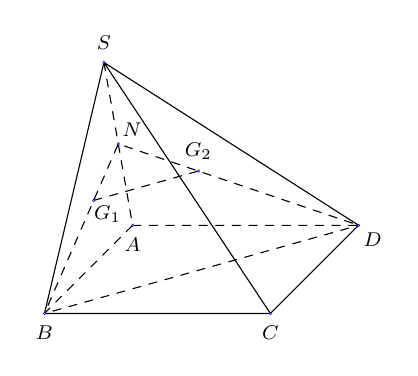
\begin{tikzpicture}[xscale=0.7,yscale=0.7,>=stealth, font=\footnotesize, line join=round, line cap=round,declare function={h=3;}]
				\path
				(0,0) coordinate (A)
				(-1.6,-1.6) coordinate (B)
				(2.5,-1.6) coordinate (C)
				(barycentric cs:A=1,C=1,B=-1)coordinate(D)
				(A)+(100:h) coordinate (S)
				(barycentric cs:S=1,A=1)coordinate(N)
				(barycentric cs:N=2,B=1)coordinate(G_1)
				(barycentric cs:N=2,D=1)coordinate(G_2)
				;
				\draw[dashed] (S)--(A)--(B)--(D) (A)--(D)--(N)--(B) (G_1)--(G_2);
				\draw (C)--(S)--(B)--(C)--(D)--(S);
				\foreach \p/\g in{A/-90,B/-90,C/-90,D/-45,S/90,N/45,G_1/-45,G_2/90}
				\shade[shading=ball](\p)circle(.03)node[shift={(\g:.25)},scale=0.9]{$\p$};
			\end{tikzpicture}
		}
	}
\end{ex}

\begin{ex}%[1H4H3-2]
	Cho hình chóp $S . A B C D$ có đáy $A B C D$ là hình thang, đáy lớn $A B$. Gọi $P$, $Q$ lần lượt là hai điểm nằm trên cạnh $S A$ và $S B$ sao cho $\dfrac{S P}{S A}=\dfrac{S Q}{S B}=\dfrac{1}{3}$. Khẳng định nào sau đây là đúng?
	\choice
	{$P Q$ cắt $(A B C D)$}
	{$P Q \subset(A B C D)$}
	{\True $P Q \parallel(A B C D)$}
	{$P Q$ và $C D$ chéo nhau}
	\loigiai{\immini{$\heva{&P Q \parallel A B \\ &A B \subset(A B C D)  \\& P Q \not \subset(A B C D)}\Rightarrow P Q \parallel(A B C D)$.}{
			\begin{tikzpicture}[scale=0.7, font=\footnotesize, line join=round, line cap=round, >=stealth]
				\def\a{5}
				\def\h{4}
				\path 	(0:0) coordinate (A)
				++(0:\a) coordinate (B)
				($(A)+(-130:\a/2)$) coordinate (D)
				($(B)+(D)-(A)$) coordinate (Ct)
				($(D)!1/2!(Ct)$) coordinate (C)
				($(A)+(90:\h)$) coordinate (S)
				(intersection of A--C and B--D) coordinate (O)
				($(S)!1/3!(A)$) coordinate (P)
				($(S)!1/3!(B)$) coordinate (Q);%giao điểm O
				\draw[dashed] 	(B)--(A)--(D)	(A)--(S) (P)--(Q);
				\draw			(B)--(C)--(D)
				(B)--(S)	(C)--(S)	(D)--(S);
				\foreach \x/\g in {A/135,B/45,C/-45,D/-135,S/90,P/-120,Q/40}
				\fill[black] 	(\x) circle (1pt)
				($(\g:3mm)+(\x)$) node {$\x$};
				%	\draw pic[draw,angle radius=2mm]{right angle=B--A--S};%Theo chiều dương
			\end{tikzpicture}}
	}
\end{ex}

\begin{ex}%[1H4H6-2]%[Dự án EX-CK1 (10,11 mới)- Lâm Chính]
	Cho hình lăng trụ $ABC.A'B'C'$. Gọi $I$ và $I'$ lần lượt là trung điểm của $AB$, $A'B'$. Qua phép chiếu song song với đường thẳng $AI'$ mặt phẳng chiếu $\left(A'B'C'\right)$ biến $I$ thành điểm nào?
	\choice
	{$A'$}
	{\True $B'$}
	{$C'$}
	{$I'$}
	\loigiai{
		\immini{
			Ta có $\heva{&{AI  \parallel B'I'} \\ &{AI=B'I'}}$.\\
			Suy ra $AIB'I'$ là hình bình hành.\\
			Vậy nên qua phép chiếu song song đường thẳng $AI'$ mặt phẳng chiếu $\left(A'B'C'\right)$ biến điểm $I$ thành điểm $B'$.
		}{
			\begin{tikzpicture}[scale=0.6, font=\footnotesize,line join=round, line cap=round, >=stealth]
				\coordinate (A) at (-2,0);
				\coordinate (B) at (-0.5,-2);
				\coordinate (C) at (2,0);
				\coordinate (H) at (1,4);
				\foreach \i in {A,B,C}{\coordinate (\i') at ($(\i)-(H)$);\draw (\i)--(\i');}
				\coordinate (I) at ($(A)!0.5!(B)$);
				\coordinate (I') at ($(A')!0.5!(B')$);
				\draw (A')--(B')--(C');
				\draw (A)--(B)--(C)--cycle (A)--(I') (B')--(I);
				\draw[dashed,thin](A')--(C') ;
				\foreach \i/\g in {A/90,B/90,C/90,A'/180,B'/-90,C'/0,I/45,I'/-120}{\draw[fill=black](\i) circle (1.5pt) ($(\i)+(\g:4mm)$) node[scale=1]{$\i$};}
			\end{tikzpicture}
		}

	}
\end{ex}

\begin{ex}%[Dự án đề cuối kỳ 1,2023-2024]%[Lê Hồng Phi]%[1D2H3-3]
	Tìm số hạng đầu $u_1$ và công bội $q$ của cấp số nhân $\left(u_n\right)$ biết $u_2=2$ và $u_5=16$.
	\choice
	{$u_1=2$, $q=2$}
	{$u_1=2$, $q=1$}
	{$u_1=-2$, $q=-1$}
	{\True $u_1=1$, $q=2$}
	\loigiai{
		Ta có $u_2=2$ và $u_5=16$, nên $u_1 \neq 0$, $q \neq 0$.\\
		Do đó $\dfrac{u_5}{u_2}=\dfrac{u_1\cdot q^4}{u_1\cdot q}=q^3 \Rightarrow q^3=8 \Rightarrow q=2$.\\
		Lại có  $u_2=u_1 \cdot q \Rightarrow u_1=\dfrac{u_2}{q}=1$.\\
		Vậy $u_1=1$, $q=2$.}
\end{ex}

\begin{ex}%[1H4H1-2]%[Dự án đề ôn tập Toán khối 11 HKI NH23-24-Dot 1-Xuan Vy Pham]%[CTST-Đề số 4]
	Hình chóp ngũ giác có bao nhiêu mặt?
	\choice
	{5}
	{4}
	{\True 6}
	{1}
	\loigiai{ \immini{Xét hình chóp ngũ giác $S.ABCDE$ có đáy là ngũ giác $ABCDE$. Dựa vào hình vẽ ta có hình chóp ngũ giác này có 6 mặt là $(SAB)$, $(SBC)$, $(SCD)$, $(SDE)$, $(SAE)$, $(ABCDE)$.}{	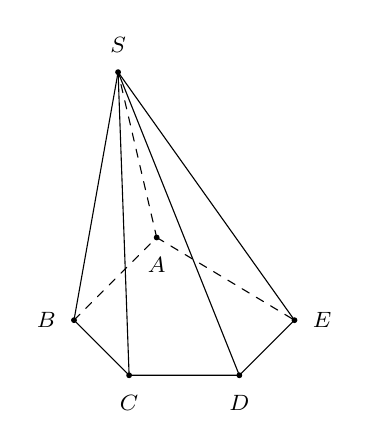
\begin{tikzpicture}[scale=0.7, font=\footnotesize, line join=round, line cap=round]
				\foreach \x\y\t in {1.5/0/A,0/-1.5/B,1/-2.5/C,3/-2.5/D,4/-1.5/E,0.8/3/S}
				\coordinate (\t) at (\x,\y);
				\draw (S)--(B)--(C)--(D)--(E)--(S);
				\draw [dashed] (B)--(A)--(S);
				\draw[dashed] (A)--(E);
				\draw (S)--(C) (S)--(D);
				\foreach \t/\g in {A/-90,B/180,C/-90,D/-90,E/0,S/90} \draw[fill=black] (\t) circle(1.2pt) node[shift={(\g:10pt)}]{$\t$};
			\end{tikzpicture} }}
\end{ex}

\begin{ex}%[1D2H1-3]%[Dự án đề ôn tập Toán khối 11 NH23-24-Đợt 1- Bùi Thanh Cương]%[CTST-Đề số 08]
	Cho dãy số $\left(u_n\right)$, biết $ u_n=2^n+1$. Mệnh đề nào sau đây đúng?
	\choice
	{$ u_1=1$}
	{$ u_2=4$}
	{$ u_3=7$}
	{\True $ u_4=17$}
	\loigiai{
		Ta có Ta có $u_1=2+1=3$; $u_2=2^2+1=5 $; 	$u_3=2^3+1=9$; $u_4=2^4+1=17$.\\
		Vậy $ u_4=17$ là mệnh đề đúng.
	}

\end{ex}

\begin{ex}%[Dự án BGK10-11,2024]%[Nguyễn Văn Nay]%[1D1H4-6]
	Cho hàm số $y=\sin x+\cos x$. Trong các khẳng định, khẳng định nào sai?
	\choice
	{$y(0)=1$}
	{Tập xác định $\mathscr{D}=\mathbb{R}$}
	{$y=\sqrt{2}\sin \left(x-\dfrac{\pi}{4}\right)$}
	{\True Tập giá trị của hàm số là $[-2;2]$}
	\loigiai{
		$y(0)=\sin 0+\cos 0 =0+1=1$.\\
		Tập xác định $\mathscr{D}=\mathbb{R}$.\\
		Ta có $\sin x+\cos x
			=\sqrt{2}\left(\dfrac{\sqrt{2}}{2}\sin x+\dfrac{\sqrt{2}}{2}\cos x\right)
			=\sqrt{2}\left(\sin x\cos \dfrac{\pi}{4}+\cos x\sin \dfrac{\pi}{4}\right)
			=\sqrt{2}\sin\left(x+\dfrac{\pi}{4}\right)$.\\
		Ta có $y=\sqrt{2}\sin\left(x+\dfrac{\pi}{4}\right)$.\\
		Ta có $-1\le \sin\left(x+\dfrac{\pi}{4}\right)\le 1
			\Rightarrow -\sqrt{2} \le \sqrt{2}\sin\left(x+\dfrac{\pi}{4}\right)\le \sqrt{2}$.\\
		Vậy Tập giá trị của hàm số là $[-\sqrt{2};\sqrt{2}]$.
	}
\end{ex}

\begin{ex}%[1H4H1-3]
	Cho hình chóp $S.ABCD$ có đáy là hình thang với đáy lớn $AB$. Gọi $M$ là trung điểm $SC$. Giao tuyến của mặt phẳng $(MAD)$ và $(SBC)$ là
	\choice
	{$ME$ (với $E$ là giao điểm của $AB$ và $CD$)}
	{\True $ME$ (với $E$ là giao điểm của $AD$ và $BC$)}
	{$SE$ (với $E$ là giao điểm của $AB$ và $CD$)}
	{$SE$ (với $E$ là giao điểm của $AD$ và $BC$)}
	\loigiai{
		\immini{Ta có $M\in(MAD)$.\\
			Mặt khác $M\in SC$, $SC\subset(SBC)$\\
			$\Rightarrow M\in(SBC)$ nên $M$ là điểm chung thứ nhất của hai mặt phẳng $(SBC)$ và $(MAD)$.\\
			Trong mặt phẳng $(ABCD)$, gọi $E=AD\cap BC$\\
			$\Rightarrow\heva{&E\in AD, \ AD\subset(MAD) \\ &E\in BC, \ BC\subset(SBC)} \Rightarrow\heva{&E\in(MAD) \\ &E\in(SBC).}$\\
			Suy ra $E$ là điểm chung thứ hai của hai mặt phẳng $(SBC)$ và $(MAD)$.\\ Vậy $ME=(MAD) \cap(SBC)$.}
		{\begin{tikzpicture}[scale=0.7,>=stealth, font=\footnotesize, line join=round, line cap=round]
				\path
				(0:0) coordinate (A)
				+(0:4) coordinate (B)
				+(-120:1.5) coordinate (D)
				+(90:3) coordinate (S)
				($(B)+(D)-(A)$) coordinate (C);
				\path ($(D)!.5!(C)$) coordinate (D);
				\path ($(S)!.5!(C)$) coordinate (M);
				\path (intersection of A--D and C--B) coordinate (E);
				\draw[dashed] (M)--(A)--(B) (C)--(D);
				\draw (E)--(M)--(D)--(S)--(A)--(E)--(B)--(S)--(C);
				\foreach \x/\g in {A/135,B/0,C/-45,D/-135,S/90,E/-90,M/45}
				\fill (\x) circle (1.5pt)
				+(\g:3.5mm) node {$\x$};
			\end{tikzpicture}}
	}
\end{ex}

\begin{ex}%[1D3H1-2]%[Dự án đề kiểm tra Toán 11 HKI NH23-24-Đợt 1- Phạm Phương]%[CTST-Đề số 5]
	%[TH]
	Giá trị của $A=\lim \limits{n \to +\infty}\dfrac{2n+1}{n-2}$ bằng
	\choice
	{$+\infty$}
	{$-\infty$}
	{\True $2$}
	{$1$}
	\loigiai{
		Ta có $A=\lim \limits{n \to +\infty}\dfrac{2n+1}{n-2}=\lim \limits{n \to +\infty}\dfrac{\dfrac{2n}{n}+\dfrac{1}{n}}{\dfrac{n}{n}-\dfrac{2}{n}}=\lim \limits{n \to +\infty}\dfrac{2+\dfrac{1}{n}}{1-\dfrac{2}{n}}=\dfrac{2+0}{1-0}=2$.
	}
\end{ex}

\begin{ex}%[1-HK1-CT-3-2324]%[VN-MT-9, Đỗ Nam]%[1H4H4-2]
	\immini{Cho hình hộp $ABCD.A'B'C'D'$. Mặt phẳng $\left(AB'D'\right)$ song song với mặt phẳng nào sau đây?
		\choice
		{$\left(BAC'\right)$}
		{$\left(BDA'\right)$}
		{$\left(ACD'\right)$}
		{\True $\left(C'BD\right)$}
	}
	{
		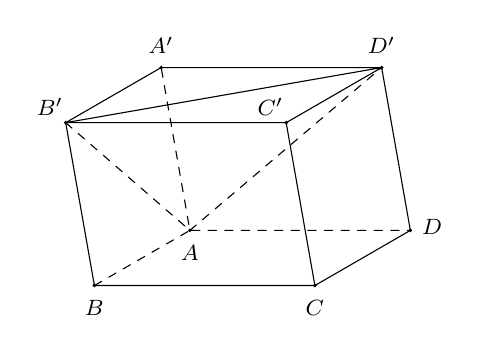
\begin{tikzpicture}[line join=round,line cap=round,>=stealth,scale=0.7,font=\footnotesize]
			%%Điểm
			\path
			(0,0)coordinate(A)++(0:4)coordinate(D)++(210:2)coordinate(C)++(180:4)coordinate(B)
			(A)++(100:3)coordinate(A')++(0:4)coordinate(D')++(210:2)coordinate(C')++(180:4)coordinate(B')
			;
			%%Cạnh
			\draw[dashed] (B)--(A)--(A') (B')--(A)--(D) (A)--(D');
			\draw (C')--(D')--(A')--(B')--(C')--(C)--(D)--(D')--(B')--(B)--(C);
			%%Hiện các điểm
			\foreach \t/\g in {A/-90,B/-90,C/-90,D/10,A'/90,B'/135,C'/135,D'/90}{
					\fill (\t) circle(1pt) node[shift={(\g:8pt)}]{$ \t $};
				}
		\end{tikzpicture}
	}
	\loigiai{
		\begin{center}
			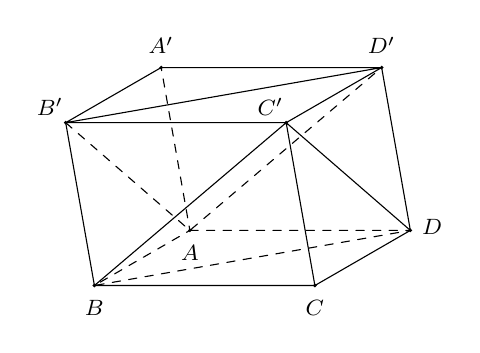
\begin{tikzpicture}[line join=round,line cap=round,>=stealth,scale=0.7, font=\footnotesize]
				\path
				(0,0)coordinate(A)++(0:4)coordinate(D)++(210:2)coordinate(C)++(180:4)coordinate(B)
				(A)++(100:3)coordinate(A')++(0:4)coordinate(D')++(210:2)coordinate(C')++(180:4)coordinate(B')
				;
				%%Cạnh
				\draw[dashed] (A)--(D)--(B)--(A)--(A') (B')--(A)--(D');
				\draw (A')--(B')--(C')--(D')--(A') (B')--(B)--(C)--(C')--(D)--(D')--(B') (D)--(C) (B)--(C');
				%%Hiện các điểm
				\foreach \t/\g in {A/-90,B/-90,C/-90,D/10,A'/90,B'/135,C'/135,D'/90}{
						\fill (\t) circle(1pt) node[shift={(\g:8pt)}]{$ \t $};
					}
			\end{tikzpicture}
		\end{center}
		Ta có $\heva{&B'D'\parallel BD\\&BD\subset \left(C'BD\right)}\Rightarrow B'D'\parallel \left(C'BD\right)$.\quad \quad (1)\\
		Đồng thời $\heva{&AD'\parallel BC'\\&BC'\subset \left(C'BD\right)}\Rightarrow AD'\parallel \left(C'BD\right)$.\quad \quad (2)\\
		Mặt khác $B'D'$, $AD'$ cùng nằm trong $\left(AB'D'\right)$.\quad\quad (3)\\
		Từ (1), (2) và (3) suy ra $\left(AB'D'\right) \parallel \left(C'BD\right)$.
	}
\end{ex}

\begin{ex}%[1D1H2-2]
	Cho $\sin \alpha=-\dfrac{3}{4}$; $\dfrac{3 \pi}{2}<\alpha<2 \pi$, giá trị của biểu thức $P=2 \sin ^2 \dfrac{\alpha}{2}+3 \cos ^2 \dfrac{\alpha}{2}$ bằng
	\choice
	{$\dfrac{12-\sqrt{7}}{4}$}
	{$\dfrac{20-\sqrt{7}}{8}$}
	{\True $\dfrac{20+\sqrt{7}}{8}$}
	{$\dfrac{12+\sqrt{7}}{4}$}
	\loigiai{$\begin{aligned} & \sin \alpha=-\dfrac{3}{4} \Rightarrow \cos \alpha= \pm \sqrt{1-\sin ^2 \alpha}= \pm \dfrac{\sqrt{7}}{4} . \\ & \text { Do } \dfrac{3 \pi}{2}<\alpha<2 \pi \Rightarrow \cos \alpha>0 \Rightarrow \cos \alpha=\dfrac{\sqrt{7}}{4} . \\ & P=2 \sin ^2 \dfrac{\alpha}{2}+3 \cos ^2 \dfrac{\alpha}{2}=2\left(\sin ^2 \dfrac{\alpha}{2}+\cos ^2 \dfrac{\alpha}{2}\right)+\cos ^2 \dfrac{\alpha}{2}=2+\dfrac{1+\cos \alpha}{2}=\dfrac{20+\sqrt{7}}{8} .\end{aligned}$
	}
\end{ex}


\begin{ex}%[1H4V1-3]
	Cho hình chóp ${S}. {ABCD}$ có đáy ${ABCD}$ là một hình thang, ${AB}\parallel {CD}$. Gọi ${I}$ là giao điểm của ${AD}$ và ${BC}$. Gọi ${M}$ là trung điểm của ${SC}$ và ${DM}$ cắt $({SAB})$ tại ${J}$. Khẳng định nào sau đây là đúng?
	\choice
	{${S}$, ${I}$, ${J}$ thẳng hàng}
	{${DM}\subset({SCI})$}
	{${DM}\subset({SAB})$}
	{\True ${SJ}=({SCD}) \cap({SAB})$}
	\loigiai{
		\begin{center}
			\begin{tikzpicture}[line join=round, line cap=round]
				\def\a{5}
				\def\h{4}
				\path 	(0:0) coordinate (A)
				++(0:\a) coordinate (B)
				($(A)+(-40:\a/2)$) coordinate (D)
				($(B)+(D)-(A)$) coordinate (Ct)
				($(D)!1/2!(Ct)$) coordinate (C)
				($(A)+(70:\h)$) coordinate (S)
				($(A)!2!(D)$) coordinate (Ax)
				($(B)!2!(C)$) coordinate (By)
				(intersection of A--Ax and B--By) coordinate (I)
				($(S)!0.5!(C)$) coordinate (M)
				($(S)+(B)-(A)$) coordinate (Sx)
				($(D)!2!(M)$) coordinate (J)
				;
				\draw[dashed] 	(A)--(B);
				\draw			(B)--(C)--(D)--(M)--(J)
				(B)--(S)	(C)--(S)	(D)--(S)--(A)--(D)--(I)--(C) (S)--(J);
				%\draw (S)--(Sx) node[above] {$x$};
				\foreach \x/\g in {A/135,B/45,C/-45,D/-135,S/90,I/0,M/180,J/60}
				\draw[fill=black] 	(\x) circle (1.5pt)
				($(\g:3mm)+(\x)$) node {$\x$};
			\end{tikzpicture}
		\end{center}
		Ta có \[J=DM\cap (SAB)\Rightarrow \heva{&J\in DM,DM\subset (SCD) \\ &J\in (SAB).}\]
		Do đó, $J\in  (SCD)\cap (SAB)$ mà $S\in (SCD)\cap (SAB)$ nên $SJ=(SCD) \cap(SAB)$.
	}
\end{ex}

\begin{ex}%[1D3V3-3]
	Tìm giá trị thực của tham số $m$ để hàm số $f(x)=\heva{&\dfrac{x^3-x^2+2x-2}{x-1} \text{ khi } x\ne 1 \\&3x+m \text{ khi } x=1}$ liên tục tại $x=1$.
	\choice
	{\True $m=0$}
	{$m=6$}
	{$m=4$}
	{$m=2$}
	\loigiai{
		Ta có $f\left(1\right)=m+3$.\\
		$\lim\limits_{x\to 1}\, f(x)=\lim\limits_{x\to 1}\, \dfrac{x^3-x^2+2x-2}{x-1}
			=\lim\limits_{x\to 1}\, \dfrac{\left(x-1\right)\left(x^2+2\right)}{x-1}
			=\lim\limits_{x\to 1}\, \left(x^2+2\right)=3$.\\
		Để hàm số $f(x)$ liên tục tại $x=1$ thì $\lim\limits_{x\to 1}\, f(x)=f\left(1\right)\Leftrightarrow 3=m+3\Leftrightarrow m=0$.
	}
\end{ex}

\TL
\begin{ex}%[2] %[Pj08-0-GK1-NH23-24--TeamTeXHoa--VoVanTu]%[1D1H5-3]
	Tìm tất cả các nghiệm của phương trình $\cos 3 x=\cos \left(\dfrac{\pi}{3}-x\right)$.
	\loigiai{
		Ta có\\ $\begin{aligned}\cos 3 x=\cos \left(\dfrac{\pi}{3}-x\right) & \Leftrightarrow\hoac{  & 3 x=\dfrac{\pi}{3}-x+k 2 \pi       \\ &3 x=x-\dfrac{\pi}{3}+k 2 \pi} \quad(k \in \mathbb{Z})\\
                                                           & \Leftrightarrow \hoac{ & 4 x=\dfrac{\pi}{3}+k 2 \pi         \\ &2 x=-\dfrac{\pi}{3}+k 2 \pi} \quad(k \in \mathbb{Z}) \\
                                                           & \Leftrightarrow\hoac{  & x=\dfrac{\pi}{12}+k \dfrac{\pi}{2} \\ &x=-\dfrac{\pi}{6}+k \pi } \quad(k \in \mathbb{Z}).\end{aligned}$\\
		Vậy phương trình có các nghiệm $x=\dfrac{\pi}{12}+k \dfrac{\pi}{2} ; x=-\dfrac{\pi}{6}+k \pi(k \in \mathbb{Z})$.
	}
\end{ex}

\begin{ex}%[Mức độ 3] %[1D3V2-5]
	Tính giới hạn sau $A=\lim\limits_{x\to 1}\dfrac{\sqrt{2x-1}-\sqrt[3]{3x-2}}{x-1}$.
	\loigiai{

		Ta có\\
		\allowdisplaybreaks
		$\begin{aligned}
				A & =\lim\limits_{x\to 1}\dfrac{\sqrt{2x-1}-\sqrt[3]{3x-2}}{x-1}                                       \\
				  & =\lim\limits_{x\to 1}\dfrac{\left( \sqrt{2x-1}-1 \right)-\left( \sqrt[3]{3x-2}-1 \right)}{x-1}     \\
				  & =\lim\limits_{x\to 1}\dfrac{\sqrt{2x-1}-1}{x-1}-\lim\limits_{x\to 1}\dfrac{\sqrt[3]{3x-2}-1}{x-1}.
			\end{aligned}$\\
		Trong đó:
		\begin{itemize}
			\item Ta có\\
			      \allowdisplaybreaks
			      $\begin{aligned}
					      \lim\limits_{x\to 1}\dfrac{\sqrt{2x-1}-1}{x-1} & =\lim\limits_{x\to 1}\dfrac{\left( \sqrt{2x-1}-1 \right)\left( \sqrt{2x-1}+1 \right)}{\left( x-1 \right)\left( \sqrt{2x-1}+1 \right)} \\
					                                                     & =\lim\limits_{x\to 1}\dfrac{2\left( x-1 \right)}{(x-1)\left( \sqrt{2x-1}+1 \right)}                                                   \\
					                                                     & =\lim\limits_{x\to 1}\dfrac{2}{\sqrt{2x-1}+1}                                                                                         \\
					                                                     & =1.
				      \end{aligned}$
			\item Ta có\\
			      \allowdisplaybreaks
			      $\begin{aligned}
					      \lim\limits_{x\to 1}\dfrac{\sqrt[3]{3x-2}-1}{x-1} & =\lim\limits_{x\to 1}\dfrac{\left( \sqrt[3]{3x-2}-1 \right)\left[ {{\left( \sqrt[3]{3x-2} \right)}^2}+\sqrt[3]{3x-2}+1 \right]}{\left( x-1 \right)\left[ {{\left( \sqrt[3]{3x-2} \right)}^2}+\sqrt[3]{3x-2}+1 \right]} \\
					                                                        & =\lim\limits_{x\to 1}\dfrac{{{\left( \sqrt[3]{3x-2} \right)}^3}-1^3}{\left( x-1 \right)\left[ {{\left( \sqrt[3]{3x-2} \right)}^2}+\sqrt[3]{3x-2}+1 \right]}                                                            \\
					                                                        & =\lim\limits_{x\to 1}\dfrac{3\left( x-1 \right)}{\left( x-1 \right)\left[ {{\left( \sqrt[3]{3x-2} \right)}^2}+\sqrt[3]{3x-2}+1 \right]}                                                                                \\
					                                                        & =\lim\limits_{x\to 1}\dfrac{3}{{{\left( \sqrt[3]{3x-2} \right)}^2}+\sqrt[3]{3x-2}+1}                                                                                                                                   \\
					                                                        & =1.
				      \end{aligned}$
		\end{itemize}
		Vậy $A=1-1=0$.
	}
\end{ex}

\begin{ex}%[1D3C1-6]%[Dự án 11 HVA 2024-2025]%[Bùi Lương Phúc]
	\immini{
		Trong hình vẽ bên, cho đường tròn $(C)$ tâm $O$, bán kính $r = 20$\,cm. Vẽ đường tròn $(C_1)$ đi qua tâm $O$ và tiếp xúc với $(C)$. Đường tròn $(C_1)$ có bán kính bằng một nửa bán kính của $(C)$, tức là $r_1 = \dfrac{r}{2} = 10$\,cm.
		Tiếp tục, vẽ đường tròn $(C_2)$ đi qua tâm của $(C_1)$ và tiếp xúc với $(C_1)$, với bán kính $r_2 = \dfrac{r_1}{2} = \dfrac{10}{2} = 5$\,cm.
		Quá trình này tiếp tục đến vô hạn, với mỗi đường tròn mới có bán kính bằng một nửa bán kính của đường tròn trước đó. Tính diện tích phần tô màu  (kết quả làm tròn đến hàng đơn vị).
	}
	{
		\begin{tikzpicture}
			\def\a{8}
			\def\b{0.5}
			\coordinate (A) at (0,0);
			\coordinate (B) at (\a,0);
			\foreach \i [count=\j from 0] in {2, 4, 8} {
					\coordinate (O\j) at ($(A)!\b^(1+\j)!(B)$);
					\fill[gray!\i0] (O\j) circle (\a/\i);
					\draw (O\j) circle (\a/\i);
					\draw (\a/\i, -\a/\i) -- (\a/\i, \a/\i);
					\fill[white] (\a/\i,-\a/\i) arc[start angle=-90, end angle=90, radius=\a/\i];
				}
			\fill[white] (\a/16,0) circle(\a/16);

			\fill[white] (\a/16,0) circle(\a/16);
			\draw[dashed] (A)--(B);
			\foreach \j/\label in {0/O, 1/O_1, 2/O_2} {
					\fill (O\j) circle(1pt) node[xshift=6pt, yshift=-6pt] {$\label$};
				}
			\fill (A) circle(1pt) node[xshift=-6pt, yshift=-6pt] {$A$};
			\fill (\a/16,0) circle(1pt) node[xshift=3pt, yshift=-6pt] {$O_3$};
		\end{tikzpicture}
	}
	\loigiai{
		Diện tích của đường tròn ban đầu $(C)$ là $S_0 = \pi r^2 = \pi \cdot 20^2 = 400\pi$\,cm$^2$.\\
		Diện tích của $(C_1)$ là $S_1 = \pi r_1^2 = \pi \cdot 10^2 = 100\pi$\,cm$^2$.\\
		Diện tích của $(C_2)$ là $S_2 = \pi r_2^2 = \pi \cdot 5^2 = 25\pi$\,cm$^2$.\\
		Tiếp tục như vậy, diện tích của các đường tròn tạo thành một cấp số nhân với số hạng đầu $S_1 = 100\pi$ và công bội $q = \dfrac{1}{4}$.\\
		Phần tô màu là tổng diện tích của các đường tròn $(C_1), (C_2), (C_3), \dots$ ngoại trừ diện tích của $(C)$. \\
		Tổng diện tích phần tô màu là tổng của một cấp số nhân lùi vô hạn
		\[
			S = S_1 + S_2 + S_3 + \dots = \dfrac{S_1}{1 - q} = \dfrac{100\pi}{1 - \dfrac{1}{4}} = \dfrac{100\pi}{\dfrac{3}{4}} = \dfrac{400\pi}{3}.
		\]
		Vậy, diện tích toàn bộ phần tô màu là
		\[
			S = \dfrac{400\pi}{3} \approx 419 \text{ cm}^2.
		\]
	}
\end{ex}

\begin{ex}%[1H4C3-6]%[Dự án đề kiểm tra Toán 11 GHKI NH23-24- Phạm Phương]%[THPT Bà Điểm-Tp HCM]
	%(3,0 điểm)
	Cho hình chóp $S.ABCD$ có đáy $ABCD$ là hình bình hành. Gọi $M$, $N$, $K$ lần lượt là trung điểm của $AB$, $AD$, $SC$.
	\begin{enumerate}
		\item Chứng minh $SA$ song song với $(KBD)$.
		\item Gọi $G$ là trọng tâm của tam giác $SBD$. Mặt phẳng $(MNG)$ cắt $SC$ tại điểm $H$. Tính tỉ số $\dfrac{SH}{SC}$.
	\end{enumerate}
	\loigiai{
		\begin{center}
			\begin{tikzpicture}[scale=1,>=stealth, font=\footnotesize, line join=round, line cap=round]
				\coordinate (A) at (0,0);
				\coordinate (B) at (-1.5,-1.8);
				\coordinate (D) at (4,0);
				\coordinate (C) at ($(B)+(D)-(A)$);
				\coordinate (S) at ($(A)+(-0.3,2.6)$);
				\path ($(A)!0.5!(B)$) coordinate (M)
				($(A)!0.5!(D)$) coordinate (N)
				($(S)!0.5!(C)$) coordinate (K)
				($(S)+(M)-(N)$) coordinate (d)
				(intersection of A--C and B--D) coordinate (O)
				($(S)!2/3!(O)$) coordinate (G)
				(intersection of A--C and M--N) coordinate (E)
				(intersection of S--C and E--G) coordinate (H)
				;
				\draw[red] ($(S)!-1.5cm!(d)$)--(d)node[above]{$d$};
				\draw (S)--(B)--(C)--(D)--cycle
				(S)--(B) (S)--(C)
				(B)--(K)--(D);
				\draw[dashed] (A)--(B) (A)--(D) (S)--(A)
				(M)--(S)--(N)--cycle
				(B)--(D)(A)--(C)
				(K)--(O)--(S)
				(M)--(G)--(N)
				(E)--(H);
				\foreach \p/\r in {S/90,A/180,B/-90,C/-45,D/0,M/180,N/-90,K/75,O/-90,G/170,H/80,E/-100}
				\fill (\p) circle (1pt) node[shift={(\r:3mm)}]{$\p$};
			\end{tikzpicture}
			\hspace*{1cm}
			\begin{tikzpicture}[scale=1,>=stealth, font=\footnotesize,line join=round,line cap=round]
				\coordinate (A) at (0,0);
				\coordinate (C) at ($(A)+(3.5,0)$);
				\coordinate (S) at (1,4);
				\path ($(A)!0.5!(C)$) coordinate (O)
				($(A)!0.5!(O)$) coordinate (E)
				($(S)!2/3!(O)$) coordinate (G)
				(intersection of S--C and E--G) coordinate (H)
				($(S)!0.5!(G)$) coordinate (I)
				($(S)!0.5!(H)$) coordinate (J)
				;
				\draw (S)--(A)--(C)--cycle
				(S)--(O)
				(A)--(J)(E)--(H)
				;
				\foreach \p/\r in {A/-145,S/90,C/45,E/-90,O/-90,H/45,J/45,I/-160,G/-20}
				\fill (\p) circle (1pt) node[shift={(\r:3mm)}]{$\p$};
			\end{tikzpicture}
		\end{center}
		\begin{enumerate}
			\item Trong hình bình hành $ABCD$ gọi $O=AC \cap BD$ suy ra $O$ là trung điểm của $AC$.
			      \\
			      $\Rightarrow KO \parallel SA$ (vì $KO$ là đường trung bình của $\triangle SAC$). \hfill (4)
			      \\
			      Mà $O\in BD \subset (KBD)$ nên $KO\subset (SBD)$ và $SA\not\subset (KBD)$.  \hfill (5)
			      \\
			      Từ (4), (5) suy ra $SA \parallel (KBD)$.
			\item Trong $(ABCD)$ gọi $E=MN\cap AC$. Khi đó $(MNG)$ cắt $SC$ tại điểm $H=EG\cap SC$.
			      \\
			      Gọi $I$, $J$ lần lượt là trung điểm của $SG$, $SH$.
			      \\
			      Ta có $\heva{&IJ\parallel HG\\& IA\parallel GE}\Rightarrow A,I,J$ thẳng hàng.
			      \\
			      Xét $\triangle ACJ$ có $EH\parallel AJ \Rightarrow \dfrac{CH}{HJ}=\dfrac{CE}{EA}=3 \Rightarrow CH=3HJ$.
			      \\
			      Lại có $SH=2HJ$ nên $SC=5HJ$. Vậy $\dfrac{SH}{SC}=\dfrac{2}{5}$.
		\end{enumerate}
	}
\end{ex}
\Closesolutionfile{ans}
